\section{Introduction}
	\subsection{Problem Background}
	There are many kinds of fungi on the earth. They are the primary decomposers of organic material in terrestrial ecosystems. Because of that, fungi are a functionally critical component of terrestrial ecosystems. Their decompose ability varys under different environment conditions and different species. To be more specific, environment conditions mainly refers to temperature and moisture and different species represents different traits like moisture tolerance, temperature tolerance, competitive rank and so on.
	
\begin{figure}[htbp]
\centering
\subfigure[Phlebia centrifuga]{
\begin{minipage}[t]{0.3\linewidth}
\centering
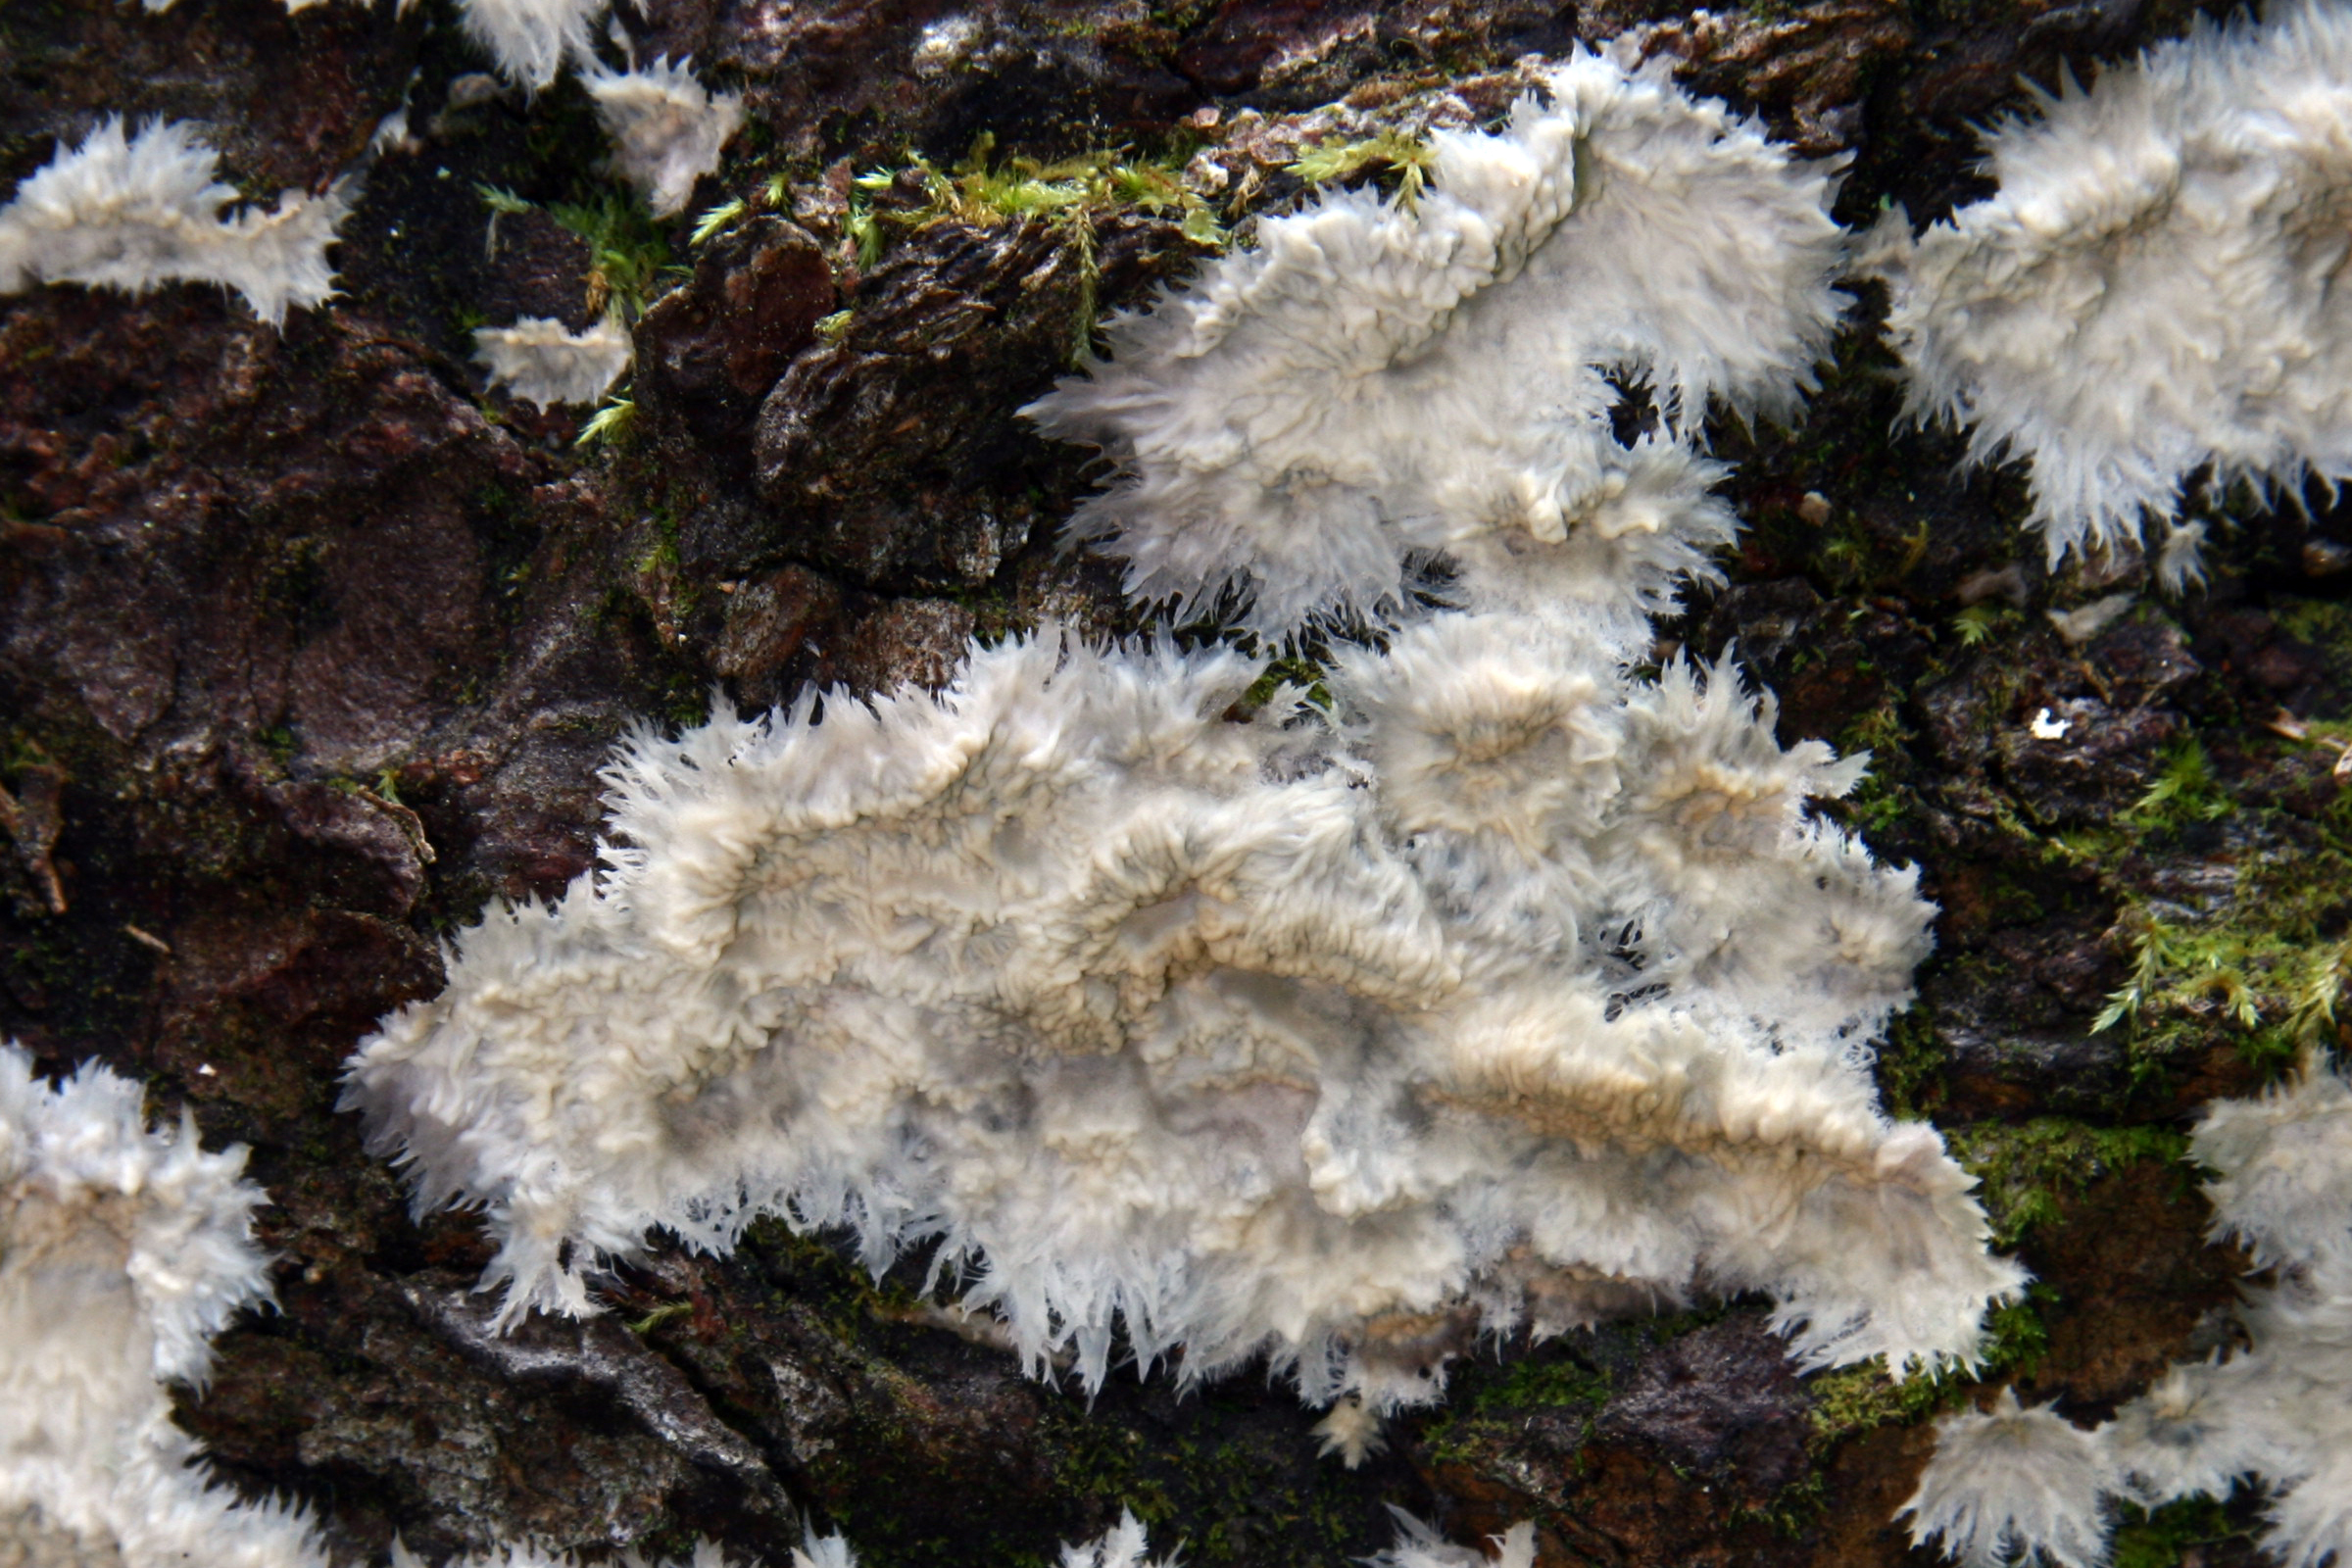
\includegraphics[width=1in]{Phlebia_centrifuga.jpg}
\end{minipage}%
}%
\subfigure[Phlebia radiata]{
\begin{minipage}[t]{0.3\linewidth}
\centering
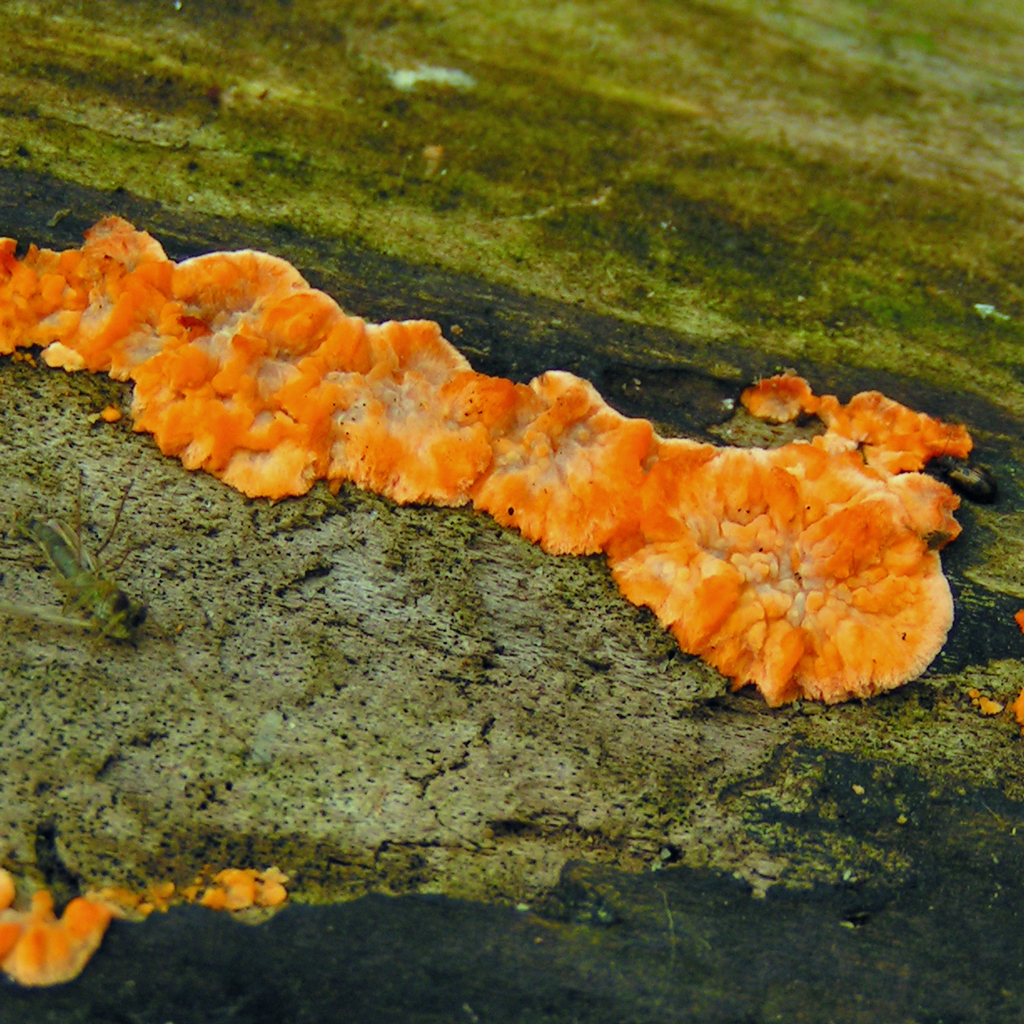
\includegraphics[width=1in]{Phlebia_radiata.jpg}
\end{minipage}%
}%
\subfigure[Hyphodontia arguta]{
\begin{minipage}[t]{0.3\linewidth}
\centering
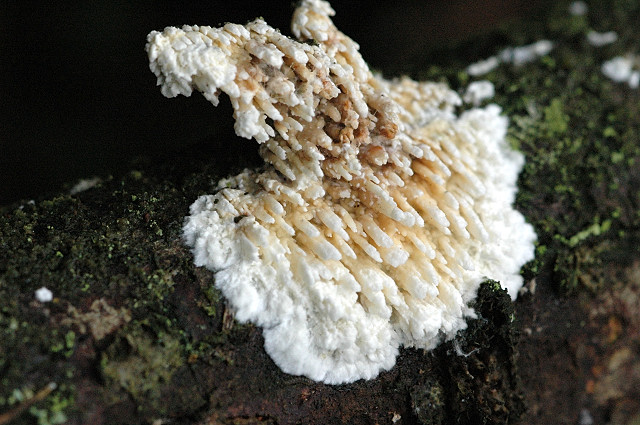
\includegraphics[width=1in]{Hyphodontia_arguta.jpg}
\end{minipage}
}%
\centering
\caption{Different Fungi}
\end{figure}

	
	\subsection{Restatement of the Problem}
	\begin{itemize}
		\item Build a mathematical model to simulate degradation process.
		\item Incoporate the interactions between different species to the previous model.
		\item Examine the sensitivity to rapid fluctuations in the environment.
		\item The advantage and disadvantage for each species under different environment
		\item Examine the importance of biodiversity
	\end{itemize}
	
	
	\subsection{Our Work}
	The topic requires us to simulate the growth of fungi community and then consider their impact on the plant material. Our work mainly includes the following:
	\begin{itemize}
		\item Based on the Competitive Lotka-Volterra equations and the data of fungi growth rate with respect to temperature and moisture, a population growth model is established.
		\item Consider the impact of plant material to fungi community to build the decomposition model.
		\item Change the climate and make rapid fluctuations to the model to discuss the outcome.
	\end{itemize}	